\documentclass{article}
\usepackage{amsmath}
\usepackage{tikz}
\usepackage{geometry}
\geometry{margin=1in}

\begin{document}

\title{Symbolic Formalization of Simulonic Field Geometry (SFG)}
\author{}
\date{}
\maketitle

\section*{Core Simulonic Field Representation}

Let the Simulonic Field Geometry (SFG) be defined by a scalar-tensor field function:
\[
\mathcal{S}(x, y, z, t) = \Phi(x, y, z, t) \cdot T_{\mu\nu}(x, y, z, t)
\]
where:
\begin{itemize}
    \item $\Phi$ is the field scalar potential
    \item $T_{\mu\nu}$ is the energy-momentum tensor of the warp spacetime
\end{itemize}

\section*{1. Octyl Component (Oscillatory Causal Topology Yield Loop)}

Octyl modulates the cyclical causal feedback loops in higher-order geometries:
\[
\mathcal{O}(t) = \alpha \cdot \sin(\omega t + \delta) \cdot e^{-\lambda t}
\]
where:
\begin{itemize}
    \item $\alpha$ is the loop amplitude
    \item $\omega$ is the causal oscillation frequency
    \item $\delta$ is the phase shift
    \item $\lambda$ is the decay constant
\end{itemize}

\section*{2. Coeternal Component (Concurrent Entangled Temporal Reciprocity)}

Coeternal defines the bidirectional temporal field equilibrium:
\[
\mathcal{C}(t) = \frac{1}{2} \left[ \mathcal{T}_f(t) + \mathcal{T}_b(t) \right]
\]
with:
\[
\mathcal{T}_f(t) = e^{i \gamma t}, \quad \mathcal{T}_b(t) = e^{-i \gamma t}
\]
This yields:
\[
\mathcal{C}(t) = \cos(\gamma t)
\]

\section*{3. Intertillage Component (Interdimensional Tillage Field)}

Defines sub-spatial cultivation patterns (analogous to domain wrinkling):
\[
\mathcal{I}(x, y) = \nabla \cdot \left[ \kappa(x, y) \cdot \vec{F}(x, y) \right]
\]
where:
\begin{itemize}
    \item $\kappa(x, y)$ is the curvature modulation field
    \item $\vec{F}(x, y)$ is the warp stress force vector
\end{itemize}

\section*{4. Delineator Component (Boundary Constraint Operator)}

Defines the boundary domain and constraints of warp field propagation:
\[
\mathcal{D} = \oint_{\partial \Omega} \vec{n} \cdot \mathcal{S} \, dA
\]
which enforces continuity of $\mathcal{S}$ across spatial boundaries $\partial \Omega$.

\section*{Combined Simulonic Field Model}

The total SFG is modeled as:
\[
\boxed{
\mathcal{S}_{\text{total}} = \mathcal{S} \cdot \left( \mathcal{O}(t) + \mathcal{C}(t) \right) + \mathcal{I}(x, y) + \mathcal{D}
}
\]

\section*{Visualization Concept (TikZ Sketch)}

\begin{center}
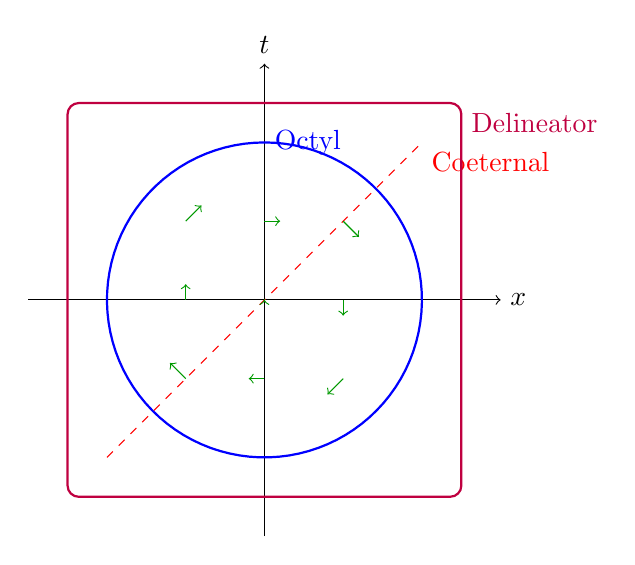
\begin{tikzpicture}[scale=1.0]
  % Axes
  \draw[->] (-3,0) -- (3,0) node[right] {$x$};
  \draw[->] (0,-3) -- (0,3) node[above] {$t$};

  % Octyl loop
  \draw[blue, thick, domain=0:360, samples=100, variable=\t]
    plot ({2*sin(\t)}, {2*cos(\t)}) node[right] {Octyl};

  % Coeternal symmetry
  \draw[red, dashed] (-2,-2) -- (2,2) node[below right] {Coeternal};

  % Intertillage vector field
  \foreach \x in {-1,0,1}
    \foreach \y in {-1,0,1}
      \draw[->, green!60!black] (\x,\y) -- ++(0.2*\y,-0.2*\x);

  % Delineator boundary
  \draw[purple, thick, rounded corners] (-2.5,-2.5) rectangle (2.5,2.5) node[below right] {Delineator};

\end{tikzpicture}
\end{center}

\end{document}
